%%%%%%%%%%%%%%%%%%%%%%%%%%%%%%%%%%%% PREAMBOLO - INIZIO %%%%%%%%%%%%%%%%%%%%%%%%%%%%%%%%%%%%%%%%%%%%%%%%%%%
\documentclass[a4paper,12pt]{report}

%%%%%%%%%%% PACCHETTI %%%%%%%%%%
\usepackage[utf8]{inputenc}
\usepackage[T1]{fontenc}
\usepackage[italian]{babel}
\usepackage{graphicx}	% per le immagini
\usepackage{fancyhdr}	% per le impostazioni della pagina
\usepackage{amsmath} %<--pacchetto American Mathematician Society
\usepackage{amssymb} %<--pacchetto piu' ampio per simboli matematici
\usepackage[pdftex,bookmarks=true]{hyperref} % per gli hyperlinks
\usepackage{boxedminipage} % for boxed paragraphs
\usepackage[usenames,dvipsnames]{color}

% PACCHETTO MOLTO CONSIGLIATO! Serve ad impostare i margini in modo professionale!
%\usepackage{layaureo}	% Il layout della tesi (richiede il pacchetto aggiuntivo LayAureo)

%pacchetto per inclusione di porzioni di codice con formattazine automatica (evita problemi sul bordo della pagina)
\usepackage{listings} 
\lstloadlanguages{C++}	%sintassi per linguaggio C++
%\lstset{frame=ltrb, framesep=5pt, , basicstyle=\scriptsize\ttfamily}
\lstset{
language=C++,
basicstyle=\footnotesize,
stringstyle=\color{Green}\ttfamily,
keywordstyle=\color{MidnightBlue}\bfseries,
morekeywords=[1]{QString, NULL, QMap, QList, QPair, qint32},
showstringspaces=true,
identifierstyle=\ttfamily\bfseries, 
commentstyle=\color{RedOrange},
captionpos=t,
columns=flexible,
aboveskip=10pt,
%backgroundcolor=\color{gray},
frame=tb,
framerule=0.2pt,
tabsize=4,
numbers=left,	%numeri di riga
numberstyle=\footnotesize	%stile dei numeri
}

%%%%%%%%%%%%%%%%%%%%%%%%%%%%%%%%

% Carattere Bitstream Character
\renewcommand{\familydefault}{bch}

% Assicura che le eventuali pagine bianche non abbiano intestazioni e pie' di pagina
\clearpage{\pagestyle{empty}\cleardoublepage}

% numerazione delle pagine "araba"
\pagenumbering{arabic}

%%%%%%%%%%%%%%%%%%%%%%%%%%%%%%%%% PREAMBOLO - FINE %%%%%%%%%%%%%%%%%%%%%%%%%%%%%%%%%%%%%%%%%%%%%%%%%%%%



%%%%%%%%%%%%%%%%%%%%%%%%%%%%%%%%% DOCUMENTO - INIZIO %%%%%%%%%%%%%%%%%%%%%%%%%%%%%%%%%%%%%%%%%%%%%%%%%%
\begin{document}
	
	% New commands
	\newcommand{\visualnetkit}{\emph{VisualNetkit}}
	\newcommand{\emulazione}{\emph{emulazione}}
	\newcommand{\linux}{\emph{Linux}}
	\newcommand{\windows}{\emph{Windows}}
	\newcommand{\testbed}{\emph{testbed}}
	\newcommand{\simulazione}{\emph{simulazione}}
	\newcommand{\virtualmachine}{\emph{Virtual Machine}}
	\newcommand{\netkit}{\emph{NetKit}}
	\newcommand{\xml}{\emph{XML}}
	\newcommand{\plugin}{\emph{Plug-In}}
	\newcommand{\stakeholders}{\emph{stakeholders}}
	\newcommand{\bu}{\emph{Bottom-Up}}
	\newcommand{\qt}{\emph{Qt}}
	\newcommand{\cpp}{\emph{C++}}
	\newcommand{\fs}{\emph{File System}}
	\newcommand{\proxy}{\emph{Proxy}}

	% alcune parole: sillabazione
	\hyphenation{up-load}
	
	% Ridefinisco localmente lo stile plain (ovvero lo stile che usa la prima
	% pagina di ogni capitolo), per nascondere il numero della
	% pagina anche all'inizio di Prefazione e Indice.
	\fancypagestyle{plain}{%
		\fancyhf{}
		\renewcommand{\headrulewidth}{0pt}
	}
	
	\addtolength{\skip\footins}{2em}	%Spaziatura testo - footnota
		
	\baselineskip=16pt	%L'interlinea 1.5 circa
	\pagestyle{empty}

	%%%%%%%%%%% FREONTESPIZIO DEDICA ED INDICE %%%%%
	\begin{figure}[!h]
	\centering
	
\includegraphics[width=3.5cm]{images/logo_uni.png}
\end{figure}
\begin{center}
	\begin{Large}Università degli studi di ``Roma Tre''\end{Large}\\
	\vspace{0.5cm}
	\begin{Large}\textbf{Facoltà di Ingegneria}\end{Large}\\
	\vspace{0.5cm}
	\begin{Large}Corso di Laurea Magistrale in Ingegneria Informatica\end{Large}\\
	\vspace{2cm}
	\begin{huge}Tesi title\end{huge}\\
	\vspace{1.5cm}
	\begin{large}Tesi finale\end{large}\\
	\vspace{2.5cm}	
	\begin{tabular}{cc}
		\begin{minipage}{6.5cm}
			\centering
			Relatore
		\end{minipage}
		&
		\begin{minipage}{6.5cm}
			\centering
			Laureando\\
		\end{minipage}
		\\
		\begin{minipage}{6.5cm}
			\centering
			\vspace{0.4cm}
			\textbf{\textit{Prof. Maurizio Pizzonia}}
		\end{minipage}
		&
		\begin{minipage}{6.5cm}
			\centering
			\textbf{\textit{Alessio Di Fazio}}
		\end{minipage}
		\\
		\begin{minipage}{6.5cm}
			\centering
			\vspace{1cm}
			Correlatore
		\end{minipage}
		\\
		\begin{minipage}{6.5cm}
			\centering
			\vspace{0.4cm}
			\textbf{\textit{Dott. Massimo Rimondini}}
		\end{minipage}
	\end{tabular}

	\vspace{1.5cm}%
	\begin{minipage}{9cm}
		\centering
		\begin{Large}Anno accademico 2007/2008\end{Large}
	\end{minipage}
\end{center}



	% inizio tesi senza intestazione di pagina e pie' di pagina
	
	\null\vspace{\stretch{1}}
\begin{flushright}
	\textit{Alla mia famiglia che mi ha dato la possibilità di laurearmi.} \\
	\textit{A me per la mia tenacia e forza di volontà.} \\
	\textit{A tutte quelle persone che non hanno mai creduto in me! :)} \\
\end{flushright}
\vspace{\stretch{1}}\null

	\tableofcontents	% l'indice
	% Inserisce la voce di questo capitolo nell'indice
	\addcontentsline{toc}{chapter}{Indice}
	
	%%%%%%%%%%%%%%%%%%%%%%%%%%%%%%%%%%%%%%%%%
	
	%%%%%%%%%%%%%%%%%%%%%%%%%%%%%%%%%%%%%%%%%
	% PREFAZIONE
	%%%%%%%%%%%%%%%%%%%%%%%%%%%%%%%%%%%%%%%%%	
	\chapter*{Introduzione}
% Inserisce la voce di questo capitolo nell'indice
\addcontentsline{toc}{chapter}{Introduzione}

Una \emph{rete di calcolatori} può essere definita come un sistema che permette la condivisione di informazioni e risorse tra un insieme di calcolatori e di apparati di rete collegati, tramite un mezzo trasmissivo.
Negli ultimi decenni si è assistito ad un eccezionale sviluppo di quella che può essere considerata la ``rete delle reti'', ovvero \emph{Internet}.
\emph{Internet} non è altro che un enorme agglomerato di sottoreti eterogenee che sono collegate con le più svariate tecnologie e che insieme costituiscono una trama capace di connettere quasi ogni luogo del pianeta. Il concetto di ``rete'' è costantemente in evoluzione e modifica profondamente, giorno dopo giorno, il mondo in cui viviamo. Si pensi alle nuove tecnologie del campo \emph{Mobile}: tutto ci conduce ad una realtà dove ogni individuo ha la possibilità di essere collegato ad \emph{Internet} ovunque si trovi.

Parallelamente è cresciuto il numero di aziende, professionisti e persone che sfruttano la \emph{Net} per svolgere le proprie attività. Questi, oltre che migliorare, integrare e fornire servizi sempre più evoluti, trasformano \emph{Internet} in un sistema attivo in continua espansione.
È per questo motivo che, fino ad oggi, molti sforzi sono stati volti alla creazione di strumenti capaci di studiare ed analizzare tutti gli aspetti che comportano la realizzazione e l'utilizzo di una rete.
Uno di questi, impiegato per lo studio delle funzionalità di una rete di calcolatori, è l'\emph{emulatore di reti}. Questi ultimi possono essere definiti come \emph{strumenti software} che riproducono in maniera esatta il funzionamento ed il comportamento dei componenti hardware che essi emulano. Gli emulatori permettono quindi di fare a meno di costose apparecchiature escludendo tutti i rischi di danneggiamento che potrebbero correre i sistemi reali durante il loro \emph{tuning}, minimizzando così l'impatto economico.
Per questi motivi tali strumenti vengono spesso utilizzati quando esiste la necessità di progettare una rete \emph{ex-novo} o di studiare le funzionalità, analizzare le architetture e testare il funzionamento di protocolli e delle configurazioni esistenti su reti reali.

La gran parte degli ambienti di emulazione esistenti risentono però di gravi debolezze che ne limitano l'utilizzo in alcune particolari realtà. Prima tra queste l'intrinseca fragilità del modello logico su cui si basano.
Questi sistemi infatti, concentrano i loro sforzi nella sempre più perfetta emulazione degli elementi coinvolti, senza curarsi della definizione di un modello formale per la rete.
Tipicamente, il modello utilizzato ricalca e forse rappresenta un'astrazione dell'emulatore su cui poggiano. Ciò comporta l'inevitabile perdita di flessibilità dell'ambiente di emulazione e l'impossibilità di definire uno schema comune per le reti emulate.

Questo lavoro offre una soluzione a tale problema proponendo un modello formale per le reti vituali emulate.
In prima istanza, è stato necessario realizzare uno studio puntuale dei vincoli introdotti dalla mancanza di uno schema adeguato. Successivamente si è proceduto alla definizione di un modello formale che fosse in grado di rappresentare le diverse reatà di interesse di una rete mantenendo intatte le doti di generalità, coerenza ed astrattezza, consone ad un modello logico.

Un'altra grave carenza di cui soffrono tali sistemi, è la scarsa flessibilità che dimostrano. Ogni ambiente infatti, dispone di una base architetturale compasta da un motore di emulazione studiato \emph{ad-hoc}, e resta ad esso irrevocabilmente vincolato.

L'ambiente realizzato nell'ambito di questo progetto supera tale vincolo grazie al modello logico su cui si centra ed alla provata certezza che un simile strumento debba collocarsi ad un livello d'astrazione superiore a quello dei sistemi di emulazione.
Per conseguire tale obiettivo è stato necessario sciogliere lo stretto legame presente tra il modello della rete e l'emulatore, astraendo e creando uno schema logico adatto alla rappresentazione di ogni rete virtuale.

Scopo primario di quest'attività di tesi è stato la realizzazione un ambiente grafico per la configurazione avanzata di reti virtuali emulate.
Tale strumento si basa su un modello comune per la realizzazione e la configurazione di reti virtuali, garantendo all'utente un'estrema usabilità e configurabilità.
Molte sono state le problematiche affrontate nel realizzare uno strumento che risultasse nel contempo estremamente flessibile ed usabile.

Il punto di forza che dona al tool caratteristiche univoche è l'adozione di una struttura modulare che poggia su di un'\emph{architettura a Plug-In}. Tale composizione ha permesso infatti, l'estensione delle funzionalità del sistema in modo assai più veloce e meno dispendioso, incrementando notevolmente caratteristiche quali flessibilità ed estensibilità.
Tuttavia questa tipologia architetturale, seppur altamente flessibile, presentava una forte limitazione per quanto concerne l'espressività dei singoli \plugin{}. 

In questo lavoro si è analizzato il problema sopra citato, trovando una soluzione che estendesse la capacità espressiva dei moduli.


Nella prima sezione si trattano i sistemi di emulazione offrendo una panoramica degli ambienti esistenti e delle specifiche funzionalità. Successivamente vengono paragonati gli ambienti di configurazione messi a disposizione dai sistemi di emulazione, enfatizzando pregi e difetti dei singoli strumenti.

Nel secondo capitolo si effettua uno studio approfondito atto a estrarre un modello che accomuni le varie configurazioni avanzate dei potenziali servizi attivi su una \virtualmachine{}. Si affontano quindi due scenari reali di configurazioni avanzate: i servizi BGP e OSPF. Lo schema risultante viene adottato mostrando la reingegnerizzazione affrontata che ha portato alla definizione del nuovo \emph{plugin framework} adottato da \visualnetkit{}.

Nella terza sezione si descrivono le fasi di progettazione e sviluppo di questo progetto, le metodologie utilizzate, le scelte realizzative e gli strumenti di supporto alle singole fasi. Si illustra in dettaglio la composizione dell'architettura, le difficoltà riscontrate e le motivazioni per le scelte effettuate.

Infine, viene proposto uno scenario reale che descrive le fasi che l'utente deve eseguire per costruire una configurazine avanzata di una rete virtuale, con l'ausilio dell'ambiente qui discusso.

		
	% Le righe seguenti impostano la struttura che avra' tutto il resto della tesi
	
	\fancypagestyle{plain}{%	% ripristino il numPag nell'ambiente plain
		\fancyhf{}
		\cfoot{\thepage}
		\renewcommand{\headrulewidth}{0pt}
	}
	% Imposto intestazione e pie' di pagina della altre pagine
	\pagestyle{fancy}	
	\rhead{\footnotesize\bfseries\leftmark}
	\lhead{\footnotesize\chaptername \ \thechapter}
	
	%%%%%%%%%%%%%%%%%%%%%%%%%%%%%%%%%%%%%%%%%
	% CAPITOLO 1
	%%%%%%%%%%%%%%%%%%%%%%%%%%%%%%%%%%%%%%%%%
	\chapter{Analisi dei requisiti}\label{capitolo:analisi}
\markboth{Analisi dei requisiti}{}
In questo capitolo di apertura verr .... bla bla

\section{Le esigenze del cliente}
Il primo passo da affrontare durante lo sviluppo .... bla bla

\subsection{I requisiti di base}
Il primo incontro con l'associazione ``Manlio~Rossi-Doria'',  .... bla bla



\subsection{Altri requisiti}
La prima versione del sistema mostrata al cliente  .... bla bla

 .... bla bla
 .... bla bla


Sono stati quindi concordati i seguenti requisiti funzionali:
\begin{itemize}
	\item	 .... bla bla
	\item	 .... bla bla
\end{itemize}



\subsection{Requisiti non funzionali}
 .... bla bla

\section{Analisi strutturale del portale esistente}
 .... bla bla

\subsection{La struttura del database e del sito di amministrazione}
 .... bla bla
	
	%%%%%%%%%%%%%%%%%%%%%%%%%%%%%%%%%%%%%%%%%
	% CAPITOLO 2
	%%%%%%%%%%%%%%%%%%%%%%%%%%%%%%%%%%%%%%%%%
	\chapter{Uno strumento orientato alla creaziene di configurazioni avanzate: l'evoluzione di \visualnetkit{}}\label{capitolo:evoluzione_visualnetkit}
\markboth{Uno strumento orientato alla creaziene di configurazioni avanzate}{}

\begin{flushright}
\begin{footnotesize}
Per ``abbracciare il cambiamento'', le strutture, il design, devono seguire le funzionalità di una applicazione in modo continuo. In un mondo in cui il cambiamento è un fattore primario e spesso violento, per seguire le funzionalità, le strutture devono essere continuamente messe in discussione e rimodellate.\\
\end{footnotesize}
\begin{footnotesize}
\textit{Francesco Cirillo}.
\end{footnotesize}
\end{flushright}

Come abbiamo introdotto nel capitolo \ref{capitolo:arte} \visualnetkit{} offre un ottima flessibilità a livello architetturale grazie alla sua struttura modulare che si appoggia su \plugin{}, ma allo stesso tempo questa malleabilità è limitata dal potere espressivo dei singoli \plugin{}. Infatti, questi possono offrire il loro contributo introducendo solamente parametri aggiuntivi espressi sotto forma di una lista di coppie chiave-valore rappresentanti le informazioni che il \plugin{} andrà ad inserire all'interno dei template\footnote{Ogni ``template'' rappresenta il contenuto testuale che andrà scritto sul file di configurazione indicato dal \plugin{} stesso; se più \plugin{} vogliono scrivere sul medesimo file di configurazione, il sistema non fa altro che accodare i vari templates.} che produrrà.

In questo capitolo discuteremo di come \visualnetkit{} sia stato profondamente modificato per dare la possibilità ai vari \plugin{} di poter ``abbracciare'' praticamente la totalità delle tipologie dei file di configurazione dei vari servizi (Dns, HTTP, E-Mail, Zebra, SSH, ecc\ldots). Si discuterà d'apprima il problema analizzando alcune configurazioni avanzate di BGP e OSPF, e da questo si cercerà di estrapolare una struttura da poter descrivere all'interno dei vari \plugin{}. Successivamente si formalizzeranno i nuovi requisiti discutendo l'impatto di tali modifiche sul sistema attuale, ed in fine ci addentreremo in uno studio di ``Analisi Architetturale'' del nuovo sistema di gestione delle properties dei \plugin{}.

\section{Il problema delle configurazioni complesse}
Quando si ha a che fare con servizi complessi come Zebra\footnote{GNU Zebra è un software opensource che gestisce i protocolli di routing basati su TCP/IP. Supporta il protocollo BGP-4 come descritto nell'RFC-1771, come anche RIPv1, RIPv2 e OSPFv2.}, quasi sempre si ha a che fare anche con file di configurazione dall'alto potere espressivo e quindi potenzialmente complessi.

Andremo ora ad analizzare da vicino due esempi di configurazioni complesse in Zebra, in particolare nei protocolli BGP\footnote{Il \emph{Border Gateway Protocol} (BGP) è un protocollo di rete usato per connettere tra loro più router che appartengono a sistemi autonomi distinti e che vengono chiamati gateway.} e OSPF\footnote{Il protocollo \emph{Open Shortest Path First} (OSPF) è uno dei protocolli di instradamento più diffusi, che gestisce le tabelle di instradamento di una rete IP con il metodo del Link State.}, e cercheremo di trovare una possibile struttura comune che possa racchiuderli.

\subsection{Configurazione avanzata in BGP}
In questa sezione cerceremo di indivinuare una struttura comune in uno scenario reale, prendendo come esempio la configurazione BGP proposta in figura \ref{figura:bgp_conf_schema}.

\begin{figure}[!htb]
	\centering
	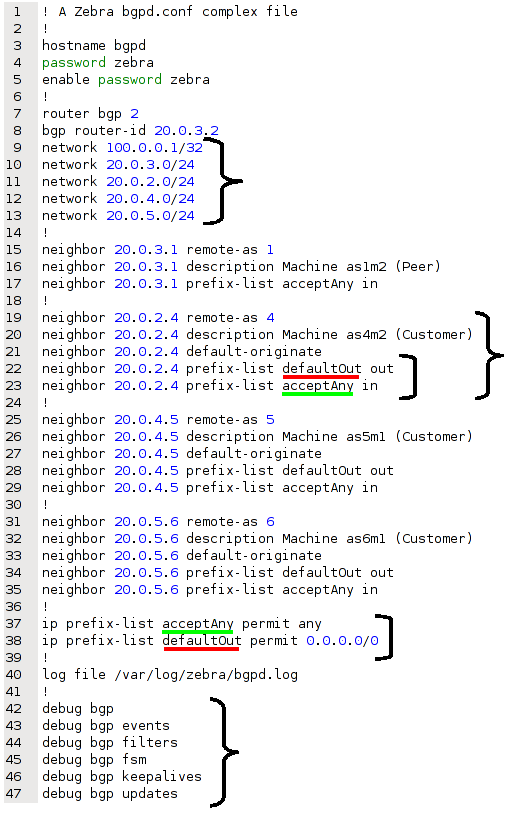
\includegraphics[width=10cm]{images/bgp_conf_schema.png}
	\caption{Una configurazione complessa di BGP.}
	\label{figura:bgp_conf_schema}
\end{figure}

Osservando la struttura del file di configurazione proposto, notiamo subito che vi è una struttura comune che può essere estrapolata e classificata. Senza considerare le righe $1\mapsto8$ che sono riconducibili ad una semplice lista di coppie chiave-valore, soffermiamoci alle righe $9\mapsto13$; qui troviamo le network annunciate dal router in questione e possiamo gia' identificare che tale struttura è una lista con cardinalità 0..n di coppie con chiave ``network'' e con valore uguale all'indirizzo IP più netmask che si vuole annunciare. Già in questo scenario una coppia chiave-valore (usata nella versione $1.0$ di \visualnetkit{}) non può essere utilizzata poiché solitamente le chiavi devono rimanere univoche.

Osserviamo ora le righe $15\mapsto35$ e soffermiamoci in particolare sulle righe $19\mapsto23$. Come descritto nella documentazione di Zebra\cite{ZEBRADOC} un ``peer'' ha la seguente sintassi:
\\
\\
\textbf{neighbor} \textit{peer} \textbf{remote-as} \textit{AS-Number}
\\
\textbf{neighbor} \textit{peer} \textbf{COMMAND}
\\
\\
dove \textbf{COMMAND} è uno dei comandi previsti da Zebra come ad esempio: \emph{description, default-originate, interface, version,} ecc\ldots nonché comandi atti al \emph{Peer Filtering} quali: \emph{discribuite-list, prefix-list, route-map,} ecc\ldots

\begin{figure}[!htb]
	\centering
	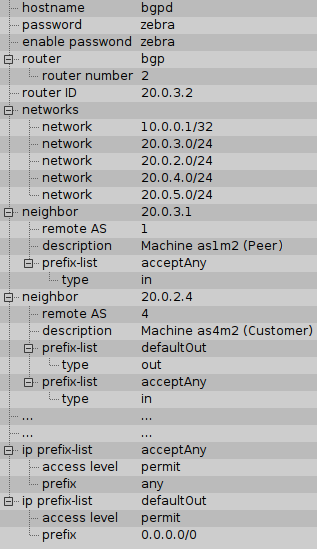
\includegraphics[width=6cm]{images/bgp_conf_tree.png}
	\caption{Configurazione complessa di BGP con struttura gerarchica.}
	\label{figura:bgp_conf_tree}
\end{figure}

Quindi, anche in questo caso è possibile raggruppare le varie definizioni dei ``vicini'' (neighbor) in una struttura gerarchica dove ogni neighbor ha una truttura composta da sotto proprietà, eventualmente con proprietà che si riferiscono a nodi esterni come nel nostro caso \emph{prefix-list} (righa $22-23$). Proprio partendo da queste due righe, possiamo identificare quindi proprietà correlate (simili al concetto di chiavi esterne in uno schema relazionale di basi di dati) a entità esterne; stiamo in definitiva affermando che quella che abbiamo davanti non è nient'altro che una struttura ad albero n-ario che possiede un enorme potere descrittivo, ma allo stesso tempo una struttura complessa da gestire e manipolare. In figura \ref{figura:bgp_conf_tree} viene mostrata la mappatura del file di configurazione in esame (figura \ref{figura:bgp_conf_schema}) in un albero n-ario.

Quella appena mostrata non è che una delle tante possibili interpretazioni di un file di configurazione in una struttura gerarchica. Solitamente ogni file di configurazione (soprattutto nei sistemi \emph{Unix like}) possiede una struttura che è riconducibile ad una con caratteristiche gerarchiche. Proprio verso questa direzione l'evoluzione che \visualnetkit{} ha avuto si è mossa, in particolare tranformando il vecchio modello chiave-valore delle proprietà dei \plugin{}, in uno altamente dinamico (con la possibilità di inserire e/o eliminare proprietà) con struttura annidata.

\subsection{Configurazione avanzata in OSPF}
Ora tenteremo di applicare quanto detto pocanzi ad un altro scenario reale che coinvolge il protocollo OSPF ed il suo file di configurazione. Prendiamo dunque in esame il file di configurazione mostrato in figura \ref{figura:ospf_conf}.

\begin{figure}[!htb]
	\centering
	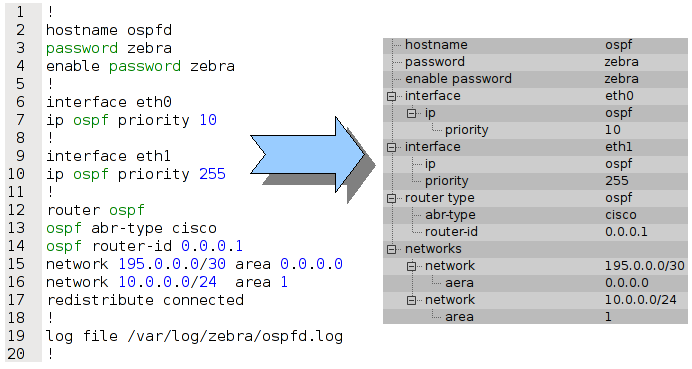
\includegraphics[width=12cm]{images/ospf_conf_schema_tree.png}
	\caption{Configurazione di OSPF e relativa vista gerarchica.}
	\label{figura:ospf_conf}
\end{figure}

Anche in questo caso possiamo procedere nel cercar di trasformare il contenuto del file di configurazione proposto, in una stuttura descritta da un albero n-ario. Iniziamo quindi ad analizzare il testo soffermandoci nelle righe $6\mapsto10$; possimo subito notare come quasta porzione abbia una struttura abbastanza uniforme - come descritto nella documentazione\cite{ZEBRADOC} - che può essere mappata all'interno di una struttura più auto descrittiva e gerarchica (figura \ref{figura:ospf_conf}).

Soffermiamoci ora sulle righe $15-16$ tralasciando le altre. In questo caso possiamo recavare una struttura ben precisa che nella documentazione di Zebra viene presentata nel seguente modo:
\\
\\
\textbf{network} \textit{a.b.c.d/m} \textbf{area} \textit{a.b.c.d}
\\
\textbf{network} \textit{a.b.c.d/m} \textbf{area} <\textit{0-4294967295}>
\\
\\
Naturalmente questi scenari sono soltanto alcuni dei tanti possibili contenuti che si possono trovare all'interno delle varie configurazioni, tuttavia abbiamo appena mostrato che qualunque siano le regole presenti nelle varie impostazioni dei servizi utilizzati, si riesce sempre a ricondurre questi ad una rappresentazione gerarchica talvolta anche complessa.

\section{Formalizzazione dei nuovi requisiti}
Prima di focalizzare gli sforzi nel trasformare il sistema in modo da essere riadattato a quanto detto fin'ora, è preferibile formalizzare i nuovi requisiti - sia quelli funzionali, che non - per avere un quadro complessivo ma charo e non ambiguo su quello che il nuovo sistema dovrà offrire. 

Si è cercato di individuare gli attori principali discutendo con gli \stakeholders{} per avere più punti vi vista. Gli attori individuati sono due:
\begin{itemize}
\item l'utente che utilizza \visualnetkit{}, in particolare uno dei suoi \plugin{};
\item l'utente/sviluppatore che desidera realizzare un \plugin{} dalle caratteristiche avanzate.
\end{itemize}
Sono stati quindi definiti una serie di scenari principali di successo per ciascun caso d'uso semplificato. L'insieme degli scenari ritenuto più importante è presentato in seguito. Si denota con il termine ``end user'' l'utente che utilizza \visualnetkit{}, e con il termine ``plugin developer'' colui che vuole realizzare un \plugin{}.

\begin{flushleft}
\begin{boxedminipage}{\textwidth}

\subsubsection*{Caso d'uso - Inizializzazione dei plugin selezionati}

\textbf{Scopo:} applicazione \visualnetkit{} \\
\textbf{Livello:} user goal \\
\textbf{Attore Primario:} End user \\
\textbf{Parti interessate e interessi:}
\begin{itemize}
\item End user: Desidera un interazione semplice, veloce ed intuitiva con il sistema per raggiungere i propri obiettivi con il minimo sforzo.
\end{itemize}

\textbf{Prerequisiti:} Il sistema deve essere avviato e l'utente deve aver creato un nuovo Lab. \\
\textbf{Goal:} L'utente ha creato un elemento base (una virtual machine, un collision domain o un link) e aver scelto ed inizializzato i \plugin{} che ha selezionato. Il sistema mostra sulla scena grafica l'elemento creato. \\

\textbf{Scenario di successo:}
\begin{enumerate}
\item l'utente seleziona dalla tool bar o dal menu la tipologia dell'elemento che intende aggiungere;
\item l'utente clicca con il mouse - tasto sinistro - un punto della scena grafica e il sistema provvede a mostrare la form per l'inizializzazione dei parametri;
\item l'utente completa la form attivando inoltre i \plugin{} che desidera siano caricati per quel determinato elemento;
\item se l'utente vuole modificare i valori di default dei \plugin{} selezionati, il sistema mostra all'utente una successiva form che offre la possibilità di modificare i vari campi delle property, nonché la possibilità di modificare la struttura delle stesse tramite l'apposito bottone ``actions'';
\item l'utente accetta e il sistema provvede a chiudere la form;
\item il sistema inizializza e aggiorna il suo stato aggiungendo l'elemento selezionato mostrandolo all'utente.
\end{enumerate}

\end{boxedminipage}
\end{flushleft}

\begin{flushleft}
\begin{boxedminipage}{\textwidth}

\subsubsection*{Caso d'uso - Modifica delle proprietà di un elemento}

\textbf{Scopo:} applicazione \visualnetkit{} \\
\textbf{Livello:} user goal \\
\textbf{Attore Primario:} End user \\
\textbf{Parti interessate e interessi:}
\begin{itemize}
\item End user: Desidera un interazione semplice, veloce ed intuitiva con il sistema per raggiungere i propri obiettivi con il minimo sforzo.
\end{itemize}

\textbf{Prerequisiti:} Il sistema deve essere avviato e l'utente deve aver creato un nuovo Lab e deve essere presente almeno un elemento base. \\
\textbf{Goal:} L'utente è riuscito con successo a modificare - contenuto o struttura - una delle proprietà di un elemento selezionato. Il sistema ha provveduto all'acquisizione dei cambiamenti modificando le proprie strutture interne.

\textbf{Scenario di successo:}
\begin{enumerate}
\item l'utente clicca due volte con il mouse - tasto sinistro - un elemento presente nella scena grafica oppure clicca una sola volta un elemento mostrato nell'insieme degli oggetti presenti, selezionandolo;
\item il sistema provvede mostrare le proprietà dell'elemento selezionato nella ``property dock'' catalogate e suddivise in base al loro ruolo: proprietà proprie dell'elemento base e proprietà offerte dai \plugin{} attivi;
\item l'utente modifica il contenuto di una proprietà. Il sistema provvede a validare il valore inserito e a registrare i cambiamenti effettuari eventualmente aggiornando gli elementi grafici;
\item l'utente vuole modificare la struttura delle proprietà di uno dei \plugin{} presenti:
	\begin{enumerate}
	\item l'utente vuole aggiungere una proprietà o sotto-proprietà dopo averne selezionata un'altra. Tramite l'apposito bottone ``actions'' l'utente può inserire altre sotto-proprietà che automaticamente il sistema propone come possibili candidate. Dopo che l'utente ha inserito una nuova proprietà, il sistema registra il cambiamento al suo interno;
	\item l'utente vuole eliminare una proprietà dopo averla selezionata. Tramite il bottone ``actions'' l'utente seleziona ``elimina proprietà'' e il sistema (validando o meno l'operazione) provvede a modificare le proprie strutture interne.
	\end{enumerate}
\end{enumerate}

\end{boxedminipage}
\end{flushleft}
Abbiamo visto i due principali scenari di successo che l'utente finale si dovrebbe aspettare, ora andremo ad analizzare altri scenari di successo che si occupano delle aspettative dell'utente (\plugin{} developer) che vuole creare un plugin offri la possibilità di impostare configurazioni avanzate per il servizio che descrive.

\begin{flushleft}
\begin{boxedminipage}{\textwidth}

\subsubsection*{Caso d'uso - Creazione di \plugin{} avanzati}

\textbf{Scopo:} \plugin{} per \visualnetkit{} \\
\textbf{Livello:} subfunction \\
\textbf{Attore Primario:} plugin developer \\
\textbf{Parti interessate e interessi:}
\begin{itemize}
\item Plugin developer: Si aspetta di riuscir a creare il proprio \plugin{} che dovrà contenere una struttura flessibile da poter descrivere la maggior parte delle configurazioni avanzate di un certo servizio offerto dal \plugin{} stesso.
\end{itemize}

\textbf{Goal:} Lo sviluppatore realizza un \plugin{} per un determinato servizio che al suo interno possiede flessibilità e alta adattabilità in modo da offrire anche configurazioni complesse.

\textbf{Scenario di successo:}
\begin{enumerate}
\item lo sviluppatore costruire il file di configurazione per il suo \plugin{} descrivendo in modo dettagliato la struttura delle proprietà;
\item lo sviluppatore crea il proprio \plugin{} che offrirà agli utenti finali la possibilità di una particolare estensione dell'elemento base su cui si basa il \plugin{};
\item il sistema provvederà a caricare il plugin durante l'avvio e ad offrire all'utente finale la possibilità di selezionarlo.
\end{enumerate}

\end{boxedminipage}
\end{flushleft}

In figura \ref{figura:uc1} viene proposto il diagramma completo dei casi d'uso e l'interazione tra essi.

\begin{figure}[!htb]
	\centering
	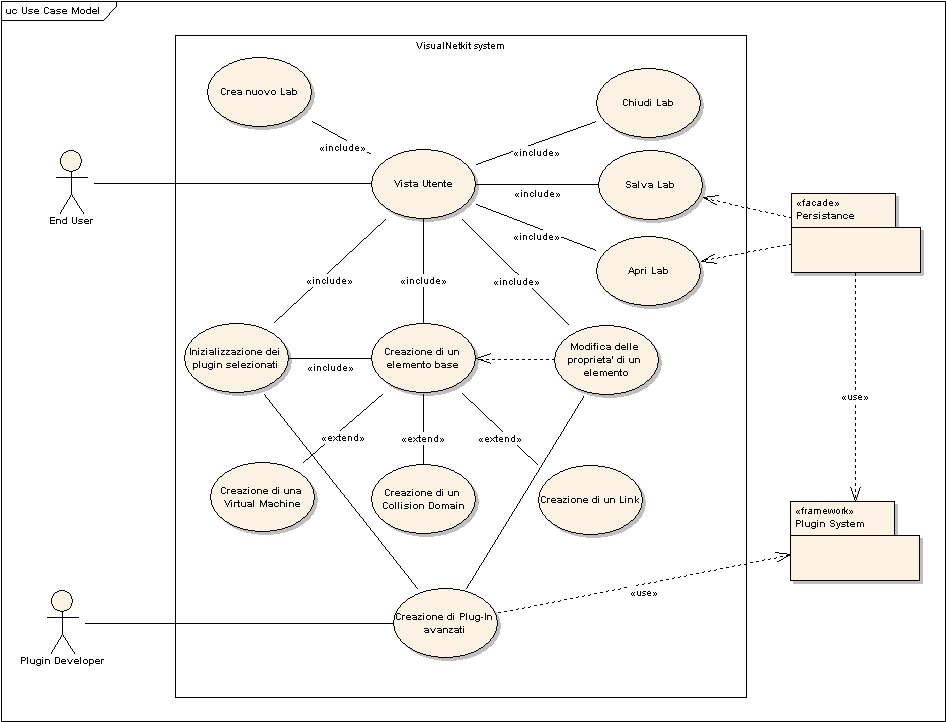
\includegraphics[width=12cm]{images/UseCaseModel.png}
	\caption{Diagramma dei casi d'uso principali in \visualnetkit{}.}
	\label{figura:uc1}
\end{figure}

\section{Analisi architetturale}

\subsection{Definizione della nuova architettura per i \plugin{}}

\subsection{Il processo di sviluppo adottato}


	
	%%%%%%%%%%%%%%%%%%%%%%%%%%%%%%%%%%%%%%%%%
	% CAPITOLO 3
	%%%%%%%%%%%%%%%%%%%%%%%%%%%%%%%%%%%%%%%%%
	\chapter{Progettazione e realizzazione}\label{capitolo:progettazione_realizzazione}
\markboth{Progettazione e realizzazione}{}
Questo capitolo è dedicato alla comprensione e descrizione delle fasi di progettazione e realizzazione di \visualnetkit{}. Si mostretà in maniera dettagliata la nuova struttura dei \plugin{} accennata nel precedente capitolo, e successivamente verrà mostrato il resto del sistema analizzando i singoli moduli che lo compongono.

\begin{figure}[!htb]
	\centering
	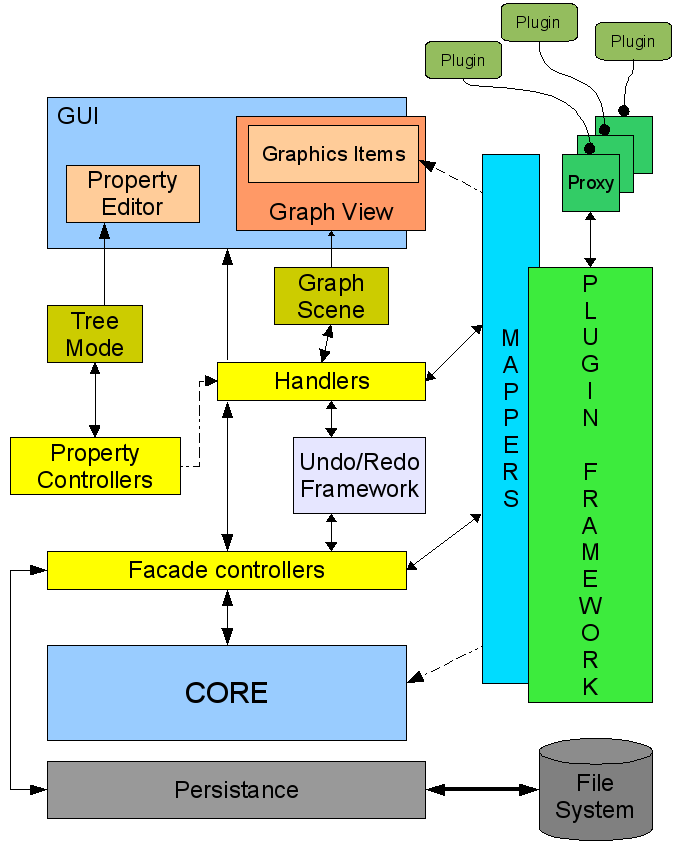
\includegraphics[width=8cm]{images/diagramma_componenti_vnetkit.png}
	\caption{Diagramma dei componenti di \visualnetkit{}}
	\label{figura:vn_componenti}
\end{figure}

In questa introduzione vogliamo subito dare al lettore un quadro generale (figura \ref{figura:vn_componenti}) della composizione architetturale nello stato attuale di \visualnetkit{}, in modo da rendere più facile la localizzazione degli elementi durante la loro trattazione.

\section{Architettura modulare basata su \plugin{}}
Come primo argomento vogliamo concentrarci sulla trattazione della struttura modulare di \visualnetkit{}, che rappresenta anche il suo punto di forza in ambito di flessibilità ed estendibilità. 

Può essere auspicabile che un software pur uso in ambito scientifico sia in possesso di funzionalità opzionali, vale a dire funzionalità che possono essere aggiunte o rimosse nel corso di una simulazione senza grossi ostacoli. Per esempio, si pensi a quanto può essere utile ad un progettista osservare il comportamento di una rete con o senza un tederminato servizio (ad esempio \emph{IPv6}) sulle macchine di cui è composta, o per uno studente quanto risulti comprensibile studiare una topologia di rete malleabile che si presta a tutti i possibili test che egli vuol effettuare.

L'utilizzo di un'architettura basata su \plugin{} dona grande flessibilità all'intero sistema ed in particolare agli utenti finali.

\subsubsection{Perché un sistema basato su \plugin{}?}
Durante le prime iterazioni e le prime fasi di testing emersero alcuni fattori di alto rischio; l'architettura era stata concepita e realizzata basandosi fortemente sul concetto che tutti i requisitivi dovevano essere assemblati staticamente nell'applicazione (come accade nei vari ambienti di configurazioni descritti nella sezione \ref{subsection:ccrc}).

Questa scelta prevedeva una lunghissima fase di sviluppo ed una continua ricerca e specifica dei requisiti e dei casi d'uso che avrebbero potuto destabilizzare l'intero sistema. Inoltre adottando questa tecnica non si sarebbe mai riusciti ad offrire una totale elasticità, ma piuttosto si sarebbe dovuto scendere a compromessi su cosa implementare e cosa no.

Analizzando meglio gli obiettivi si è giusti alla conclusione che l'unica strada percorribile fosse quella che prevedeva la trasformazione dell'architettura in una modularizzata. Il core del sistema (senza alcun \plugin{} attivo) avrebbe offerto all'utente solamente la possibilità di creare una rete a livello topologico, priva quindi di caratteristiche proprie.

Questa nuova tecnica avrebbe da un lato offerto una sicura controllabilità dei fattori di rischio, restringendoli alla re-ingegnerizzazione del sistema per renderlo modulare, dall'altro avrebbe reso \visualnetkit{} estremamente scalabile e flessibile e gli avrebbe conferito una connotazione del tutto unica nel suo genere.

\subsection{Interazione tra sistema e \plugin{}}
Quando si sviluppa un'applicazione che si basa fortemente su \plugin{} la cosa più importante è definire i confini dell'uno e dell'altro sistema. In poche parole ambiente e moduli devono essere ben descritti per non imbattersi in fenomei di sovrapposizione; questi due mondi devono cooperare, ma non devono intralciarsi né tantomeno svolgere le stesse mansioni.

Dopo un'attenta ed accurata fase di studio si è arrivati a definire la linea di demarcazione tra il sistema e le estensioni. I vari \plugin{} possono essere attivati sugli elementi di base del sistema offrendo una sorta di caratterizzazione più specifica. Su di un elemento possono essere attivi contemporaneamente più \plugin{} che di fatto donano una definizione ben precisa all'elemento. Se per esempio su un host noi attiviamo \plugin{} quali DNS e HTTP, balza subito all'occhio il tipo di quell'oggetto; abbiamo semplicemente di fronte una macchina virtuale che offre un servizio di DNS e che allo stesso tempo è un server Web di qualche tipo.

Andiamo ora a descrivere in dettaglio la struttura del sotto sistema che permette ai moduli di colloquiare con il core dell'applicazione e la definizione delle varie interfaccie - figura \ref{figura:uml_plugin_framework}.

\begin{figure}[!htb]
	\centering
	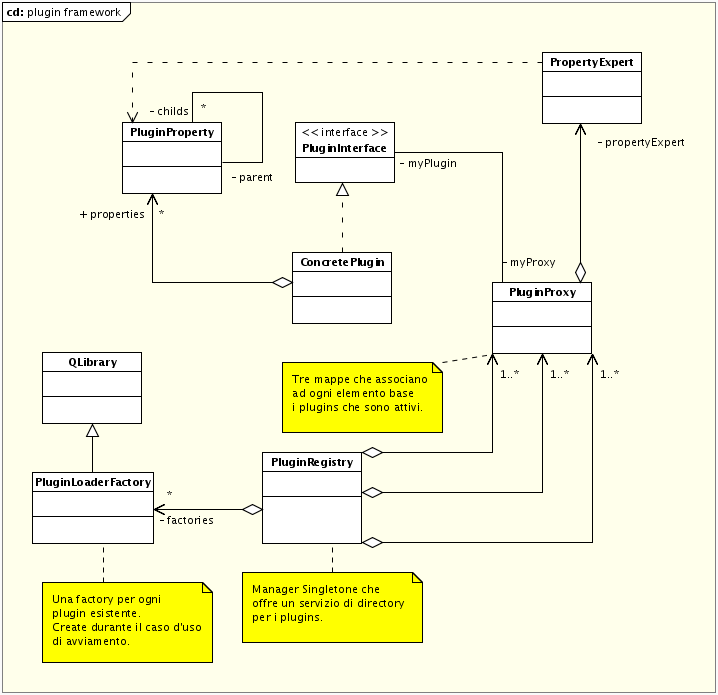
\includegraphics[width=12cm]{images/plugin_framework_uml.png}
	\caption{Diagramma delle classi del sotto sistema di gestione dei \plugin{}.}
	\label{figura:uml_plugin_framework}
\end{figure}



\section{Elementi architetturali}

\subsection{L'interfaccia utente}


\subsection{Gli handlers}

\subsection{Property controllers}

\subsection{Undo Framework}

\subsection{Elementi del dominio}

\subsection{L'accesso al \fs{}}

\subsection{I mappers}

\section{La gestione avanzata delle properties}
\subsection{Properties di base}
\subsection{Properties dei \plugin{}}

\section{Strumenti di supporto allo sviluppo}
\subsection{Il framework \qt{}}
\subsection{Altri strumenti secondari}

	
	%%%%%%%%%%%%%%%%%%%%%%%%%%%%%%%%%%%%%%%%%
	% CAPITOLO 4
	%%%%%%%%%%%%%%%%%%%%%%%%%%%%%%%%%%%%%%%%%
%	\chapter{Scenari per la configurazione avanzata di reti virtuali}\label{capitolo:esempi}
\markboth{Scenari per la configurazione avanzate di reti virtuali}{}

I precedenti capitoli hanno descritto il lavoro svolto durante l'attività di tesi. In questo capitolo si vuole illustrare il funzionamento dell'ambiente sviluppato, suddividendo l'esposizione in uno scenario reale descritto in tre fasi.


\section{Caso di studio: realizzazione e configurazione di un Lab tramite \visualnetkit{}}
Il primo di questi relaziona i passi da effettuare per la costruzione di un semplice laboratorio composto da una rete LAN.

Lo step successivo descrive le mansioni da eseguire sul laboratorio precedentemente cerato per riuscire a configurare i nodi presenti, secondo le esigenze dell'utente. In questo vengono quindi mostrate le potenzialità del nuovo \plugin{} framework, sottolineando com'è possibile applicare dettagliatamente le configurazioni. In mancanza di moduli complessi - come \emph{Zebra} o \emph{Quagga} -, è stato utilizzato un \plugin{} di test che possiede una struttura delle properties estesa e altamente dinamica, priva di un significato logico.

L'ultima parte espone alcuni test di funzionamento sulla rete precedentemente realizzata, tramite l'ausilio dell'ambiente di emulazione offerto da \netkit{}.

\subsection{Realizzazione di un laboratorio}
L'obiettivo di questa fase di apertura è la realizzazione di una topologia di rete semplice composta da quattro \virtualmachine{} connesse a stella ad un unico dominio di collisione.

Per prima cosa occorre creare un nuovo laboratorio scegliendo dal menu \emph{File} la voce \emph{New Lab}, oppure tramite l'uso della shortcut \textbf{Ctrl+N}. Da questo momento fino alla chiusura del Lab, \visualnetkit{} è pronto per la creazione della rete. In figura \ref{figura:vn_ex_dock} è discritta la struttura delle docks che compongono l'interfaccia utente.

\begin{figure}[!htb]
	\centering
	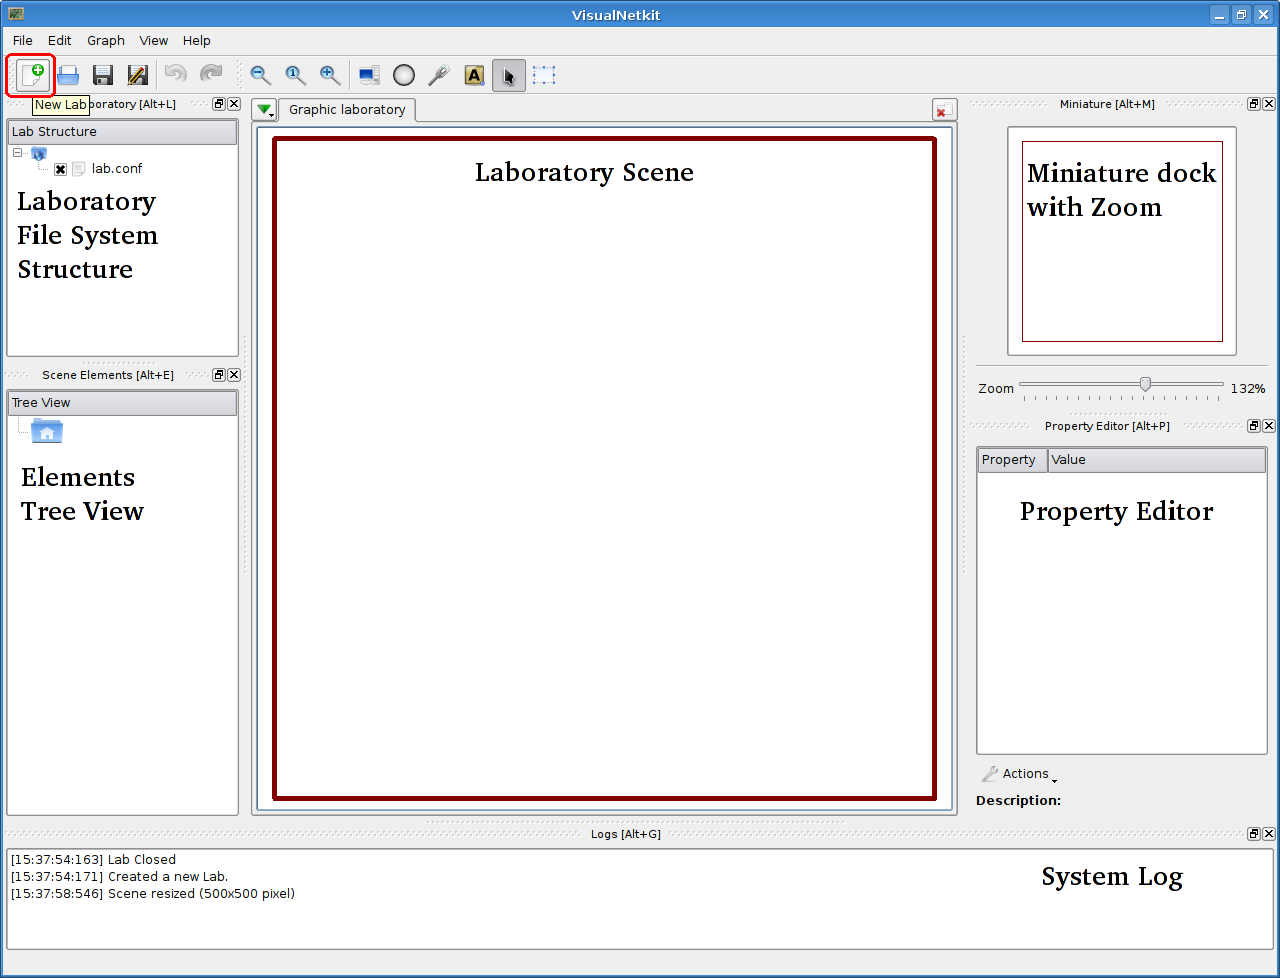
\includegraphics[width=12.5cm]{images/vnetkit_example1.png}
	\caption{Docks in \visualnetkit{}}
	\label{figura:vn_ex_dock}
\end{figure}

Le docks presenti - che comprendono anche le tool-bars -, sono tutte configurabili. L'utente può comodamente disporle a suo piacimento, nonché nascondere quelle che ritiene superflue.

Successivamente è possibile iniziare a costruire la topologia della rete in esame: utilizzando le apposite azioni presenti nel menu \emph{Graph}, l'utente può inserire nella scena grafica elementi quali Virtual Machines, Links, Collision Domain e Aree. Dapprima inseriamo le quattro \virtualmachine{} nella scena, attivando per l'host ``PC1'' anche il \plugin{} \emph{Test} che verrà configurato in un secondo momento.

\begin{figure}[!htb]
	\centering
	\includegraphics[width=12cm]{images/vnetkit_example3.png}
	\caption{Inserimento dei links.}
	\label{figura:vn_ex_links}
\end{figure}

Al termine dell'operazione è possibile inserire il dominio di collisione posto a ``centro stella'', che andrà a collegare tutti gli host virtuali precedentemente creati. In fine, il lavoro sarà completato dall'inserimento dei links in cui verranno attivati i \plugin{} \emph{IPv4} e \emph{MAC}. Figura \ref{figura:vn_ex_links}.

Una volta realizzata la topologia di rete desiderata, il tool permette l'aggiunta di aree che possono essere utilizzate come etichette, oppure come aggregatori di elementi.

\subsection{Configurazione avanzata del laboratorio}
L'utente spesso ha la necessità di configurare i servizi presenti all'interno degli host virtuali per garantire un corretto funzionamento delle macchine, per effettuare con successo i test desiderati. \visualnetkit{} offre questa possibilità mediante l'uso della dock delle proprietà.
Quando si seleziona un elemento della scena grafica - doppio click -, il sistema provvede a renderizzare le informazioni dell'oggetto all'interno della property dock. Possiamo quindi trovare tutte le propietà presenti all'interno dei \plugin{} attivi per l'entità selezionata.

Alcuni moduli più complessi (nel caso dell'esempio il \plugin{} \emph{Test}) prevedono la possibilità di poter manipolare la struttura delle properties, in particolare questo avviene inserendo o eliminando sotto-attributi (figura \ref{figura:vn_ex_pp}).

\begin{figure}[!htb]
	\centering
	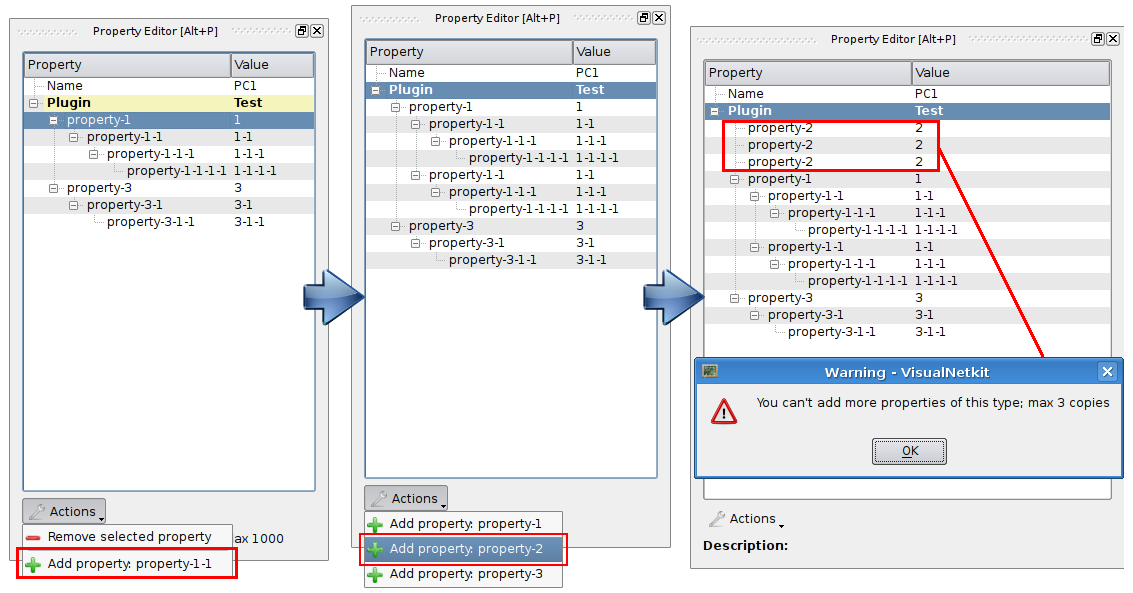
\includegraphics[width=13cm]{images/vnetkit_property_evolution.png}
	\caption{Modifica della struttura delle properties di un \plugin{}.}
	\label{figura:vn_ex_pp}
\end{figure}
Si vuole quindi modificare la struttura del modulo \emph{Test} attivo sulla macchina virtuale ``PC1''. Come mostrato, viene prima inserata una sotto-proprietà dell'attributo ``property-1'', successivamente si tenta di inserire tre copie della proprietà ``property-2'' che il modulo prevede.
Al tentativo di inserimento della quarta copia di quest'ultima, il \plugin{} restituisce un errore in quanto non sono previste più di tre duplicati per la proprietà in esame.

Tramite l'apposito bottone ``Actions'' è possibile, per ogni proprietà di un modulo, eliminare o aggiungere le sotto-property quando consentito. Quest'ultimo controllo - come quello inerente al controllo di cardinalità di una property poc'anzi citato -, è interamente affidato al \plugin{}.

Il modulo analizzato nell'esempio è puramente utilizzato per il testing. Tuttavia si può facilmente immaginare che un \plugin{} complesso, come \emph{Zebra} o \emph{Quagga}, possa avere una struttura simile a quella mostrata che contiene molteplici attributi e sotto-attributi.

\subsection{Sperimentazioni sul laboratorio esportato}
Lo stadio finale della costruzione di un laboratorio mediante l'utilizzo di \visualnetkit{} si conclude con il salvataggio dello stesso sul \fs{}. Mediante la voce \emph{Save As\ldots} presente nel menu \emph{File} è possibile selezionare la directory dove il Lab creato verrà esportato.

\begin{figure}[!htb]
	\centering
	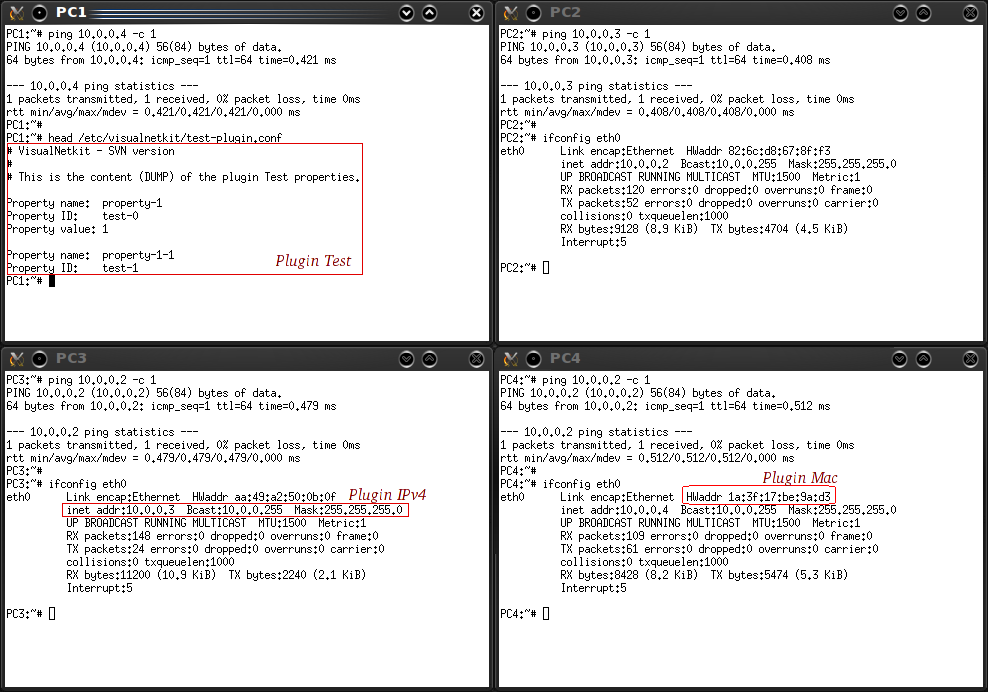
\includegraphics[width=13cm]{images/netkit_lab_example.png}
	\caption{Il laboratorio avviato emulato tramite \netkit{}.}
	\label{figura:ex_netkit}
\end{figure}

Effettata questa operazione si può provvedere anche alla chiusura di \visualnetkit{}. Da questo momento in poi viene utilizzato \netkit{}\footnote{La spiegazione di come avviare un laboratorio con \netkit{} va oltre gli obiettivi di questo lavoro.} per avviare la rete virtuale, dove è possibile effettuare tutti i test che si desiderano.

Studiando il comportamento della rete precedentemente creata, è possibile osservare che il laboratorio esportato è completo in ogni dettaglio. Tutte gli host virtuali, connessi ad un unico dominio di collisione, riescono a colloquiare correttamente, come mostrato in figura \ref{figura:ex_netkit}. Inoltre si può constatare che i \plugin{} attivati sui links e sull'host ``PC1'' hatto tutti contribuito a caratterizzare la parte della rete di propria competenza.

Ancora, è possibile immaginare un'estensione dell'architettura al fine di prevedere la possibilità di avviare un laboratorio direttamente da \visualnetkit{} avendo la possibilità di mostrare all'utente una rappresentazione grafica dei terminali virtuali.

In ultima instanza, potrebbe risultare necessaria ed innovativa la realizzazione di un meccanisco che permetta ai vari moduli di comunicare e cooperare tra di loro. Si pensi ad esempio, allo scenario in cui un modulo (attivo su una \virtualmachine) volesse conoscere tutti gli indirizzi IPv4 attivi sulle interfacce hardware presenti sull'host.

	
	%%%%%%%%%%%%%%%%%%%%%%%%%%%%%%%%%%%%%%%%%
	% CAPITOLO 5
	%%%%%%%%%%%%%%%%%%%%%%%%%%%%%%%%%%%%%%%%%
%	\include{capitoli/cap5}
	
	%%%%%%%%%%%%%%%%%%%%%%%%%%%%%%%%%%%%%%%%%
	% CONCLUSIONI
	%%%%%%%%%%%%%%%%%%%%%%%%%%%%%%%%%%%%%%%%%
	% Elimino l'intestazione della pagina per le conclusioni e la bibliografia
	\rhead{}
	\lhead{}	
	\renewcommand{\headrulewidth}{0pt}
	
	\chapter*{Conclusioni}
% Inserisce la voce di questo capitolo nell'indice
\addcontentsline{toc}{chapter}{Conclusioni}

 .... bla bla\footnote{baobao!}
ciao

L'aggiornamento globale di un portale web L'aggiornamento globale di un portale web L'aggiornamento globale di un portale web L'aggiornamento globale di un portale web L'aggiornamento globale di un portale web L'aggiornamento globale di un portale web L'aggiornamento globale di un portale web L'aggiornamento globale di un portale web L'aggiornamento globale di un portale web L'aggiornamento globale di un portale web L'aggiornamento globale di un portale web L'aggiornamento globale di un portale web L'aggiornamento globale di un portale web L'aggiornamento globale di un portale web L'aggiornamento globale di un portale web L'aggiornamento globale di un portale web L'aggiornamento globale di un portale web L'aggiornamento globale di un portale web L'aggiornamento globale di un portale web L'aggiornamento globale di un portale web L'aggiornamento globale di un portale web L'aggiornamento globale di un portale web L'aggiornamento globale di un portale web L'aggiornamento globale di un portale web
 .... bla bla
	
	%%%%%%%%%%%%%%%%%%%%%%%%%%%%%%%%%%%%%%%%%
	% RINGRAZIAMENTI
	%%%%%%%%%%%%%%%%%%%%%%%%%%%%%%%%%%%%%%%%%
	\chapter*{Ringraziamenti}
% Inserisce la voce di questo capitolo nell'indice
\addcontentsline{toc}{chapter}{Ringraziamenti}

A Michela per il suo impagabile sostegno e aiuto.\\
A tutti gli amici con i quali ho condiviso questi anni universitari.\\
A Dario per avermi fatto avvicinare al mondo open-source.\\
Al Prof. Maurizio Pizzonia e Massimo Rimondini che mi hanno dato la possibilità di svolgere questo lavoro.\\
Ed infine, a tutti i professori del Dipartimento di Informatica e Automazione (\emph{D.I.A.}) dell'Università degli studi di ``Roma Tre'', che con estrema professionalità hanno sempre svolto il proprio lavoro egregiamente.

	
	%%%%%%%%%%%%%%%%%%%%%%%%%%%%%%%%%%%%%%%%%
	% BIBLIOGRAFIA
	%%%%%%%%%%%%%%%%%%%%%%%%%%%%%%%%%%%%%%%%%
	\clearpage
% Inserisce la voce di questo capitolo nell'indice
\addcontentsline{toc}{chapter}{Bibliografia}
\begin{thebibliography}{9}
\bibitem{OSSINI}
	M. Zec, M. Mikuc.
	\emph{Operating System Support for Integrated Network Emulation in IMUNES}, to appear in Proceedings of the 1st Workshop on Operating System and Architectural Support for the on demand IT InfraStructure / ASPLOS-XI, Boston, October 2004.

\bibitem{MVNL08}
	Jean-Vincent Loddo, Luca Saiu.
	\emph{Marionnet: A Virtual Network Laboratory and Simulation Tool}, SimulationWorks, Marseille (France), 2008

\bibitem{IMUNESHOWTO}
	Gabriel Astudillo Mu\~{n}oz.
	\emph{Descripcíon del software IMUNES para su utilizacíon en el Laboratorio de Redes y Sistemas Operativos}, www.elo.utfsm.cl/\verb+~+elo324/doc/manual\verb+_+imunes.pdf.

\bibitem{QUATC05}
	Fabrice Bellard.
	\emph{QEMU, a Fast and Portable Dynamic Translator}, 2005 USENIX Annual Technical Conference.

\bibitem{VNUMLT}
	\emph{VNUML Tutorial}, www.dit.upm.es/vnumlwiki/index.php/Tutorial.

\bibitem{VNUMLGUI}
	\emph{VNUMLGUI}, pagesperso.erasme.org/michel/vnumlgui.

\bibitem{NETKIT}
	\emph{Netkit}, www.netkit.org.

\bibitem{ZEBRADOC}
	\emph{Zebra Documentation}, www.zebra.org/zebra/index.html

\bibitem{IRPI07}
	Massimo Rimondini.
	\emph{Interdomain Routing Policies in the Internet: Inference and Analysis}, A thesis presented by Massimo Rimondini in partial fulfillment of the requirements for the degree of Doctor of Philosophy in Computer Science and Engineering, Roma Tre University, Dept. of Informatics and Automation, March 2007.

\bibitem{ECNN07}
	Massimo Rimondini.
	\emph{Emulation of Computer Networks with Netkit}, Tutorial held during the 4th International Workshop on Internet Performance, Simulation, Monitoring and Measurement (IPS MoMe 2006) in Salzburg, February 2006.

\bibitem{AUPL04}
	Craig Larman.
	\emph{Applying UML and Patterns: An Introduction to Object-Oriented Analysis and Design and Iterative Development (3rd Edition)}, Prentice Hall PTR, October 2004.

\bibitem{SSA06}
	Nick Rozanski, Eoin Woods
	\emph{Software System Architecture: Working With Stakeholders Using Viewpoints and Prespectives}, Addison Wesley

\end{thebibliography}

	
\end{document}

%%%%%%%%%%%%%%%%%%%%%%%%%%%%%%%%% DOCUMENTO - FINE %%%%%%%%%%%%%%%%%%%%%%%%%%%%%%%%%%%%%%%%%%%%%%%%%%
